
\title{T-61.5130 Machine Learning and Neural Networks}
\author{Karhunen, Luttinen}
\date{Exercise 2, ??.??.2012}


% \usepackage{subfigure}
% \usepackage{epsfig}
% \usepackage{amsmath}
% \parindent 0mm
% \textwidth 16cm
% \textheight 23cm
% \oddsidemargin 0cm
% \evensidemargin 0cm
% \topmargin -10mm
\newcommand{\vect}[1]{{\bf{#1}}}
\newcommand{\svect}[1]{\boldsymbol{#1}}
\newcommand{\matr}[1]{\boldsymbol{#1}}
\newcommand{\vw}{{\bf{w}}}
\newcommand{\ve}{{\bf{e}}}
\newcommand{\vx}{{\bf{x}}}

\begin{document}

\maketitle

\begin{enumerate}

\item Let the error function be
  \begin{equation*}
    {\cal E}(\mathbf{w})=w_1^2+10w_2^2,
  \end{equation*}
  where $w_1$ and $w_2$ are the components of the two-dimensional
  parameter vector $\mathbf{w}$. Find the minimum value of ${\cal
    E}(\mathbf{w})$ by applying the steepest descent method. Use
  $\mathbf{w}(0)=[1,1]^T$ as an initial value for the parameter vector
  and the following constant values for the learning rate:
  \begin{enumerate} \item $\alpha=0.04$ \item $\alpha=0.1$ \item
    $\alpha=0.2$
  \item What is the condition for the convergence of this method?
  \end{enumerate}

  \begin{solution}

    The error function is
    \begin{equation*}
      {\cal E}(\vw)=w_1^2+10w_2^2,
    \end{equation*}
    where $w_1$ and $w_2$ are the components of the two-dimensional
    parameter vector $\vw$. 

    The gradient is
    \begin{equation*}
      \nabla_{\vw} {\cal E} (\vw) = \begin{pmatrix} \frac{\partial {\cal E}
          (\vw)}{\partial w_1} \\  \frac{\partial  {\cal E} (\vw) }{\partial
          w_2}\end{pmatrix} = \begin{pmatrix} 2 w_1 \\  20 w_2 \end{pmatrix}.
    \end{equation*}

    The steepest descent method has a learning rule:
    \begin{equation*}
      \begin{split}
        \vw(n+1) & = \vw(n)- \alpha \nabla_{\vw(n)} {\cal E} (\vw(n)) \\
        & = \begin{pmatrix} w_1 \\  w_2 \end{pmatrix} - \alpha
        \begin{pmatrix} 2 w_1 \\  20 w_2 \end{pmatrix} = \begin{pmatrix}
          (1 - 2 \alpha) w_1 \\  (1 - 20 \alpha) w_2 \end{pmatrix} .
      \end{split}
    \end{equation*}

    It was given $\vw(0) = \begin{pmatrix} 1 & 1 \end{pmatrix}^T$:
    \begin{equation*}
      \vw(n+1) = \begin{pmatrix} (1 - 2 \alpha)^{n+1} w_1(0) \\  (1 - 20
        \alpha)^{n+1} w_2(0) \end{pmatrix} = \begin{pmatrix} (1 - 2
        \alpha)^{n+1} \\  (1 - 20 \alpha)^{n+1} \end{pmatrix}. 
    \end{equation*}

    \begin{enumerate}
    \item $\alpha = 0.04$: 
      \begin{equation*}
        \vw(n+1) = \begin{pmatrix} 0.92^{n+1} \\
          0.20^{n+1} \end{pmatrix} \xrightarrow[n\rightarrow\infty]{}\begin{pmatrix}0\\0\end{pmatrix}
      \end{equation*}

    \item $\alpha = 0.1$: 
      \begin{equation*}
        \vw(n+1) = \begin{pmatrix} 0.8^{n+1} \\
          (-1)^{n+1} \end{pmatrix} \xrightarrow[n\rightarrow\infty]{}\left\{\begin{array}{cl}\begin{pmatrix}0\\-1\end{pmatrix} & \mbox{,when } n\mbox{ is even}\\
            \begin{pmatrix}0\\1\end{pmatrix} & \mbox{,when } n\mbox{ is odd}\end{array}\right.
      \end{equation*}

    \item $\alpha = 0.2$: 
      \begin{equation*}
        \vw(n+1) = \begin{pmatrix} 0.6^{n+1} \\
          (-3)^{n+1} \end{pmatrix} \xrightarrow[n\rightarrow\infty]{}\left\{\begin{array}{cl}\begin{pmatrix}0\\-\infty\end{pmatrix} & \mbox{,when } n\mbox{ is even}\\
            \begin{pmatrix}0\\\infty\end{pmatrix} & \mbox{,when } n\mbox{ is odd}\end{array}\right.
      \end{equation*}

    \item Iteration converges if $| 1 - 2 \alpha | < 1$ and $| 1 - 20 \alpha | < 1 \Rightarrow 0 < \alpha < 0.1$. 
      No oscillations occur if $0 < 1 - 2 \alpha < 1$ and $0 < 1 - 20 \alpha < 1 \Rightarrow 0 < \alpha < 0.05$.

    \end{enumerate}

  \end{solution}

\item The normalized LMS algorithm is described by the following
  recursion for the weight vector:
  \begin{equation*}
    \Hat{\mathbf{w}}(n+1)= \Hat{\mathbf{w}}(n) +\frac{\eta e(n)
      \mathbf{x}(n)} {\| \mathbf{x}(n) \|^2},
  \end{equation*}
  where $\eta$ is a positive constant and $\|\mathbf{x}(n) \|$ is the
  Euclidean norm of the input vector $\mathbf{x}(n)$. The error
  signal $e(n)$ is defined by
  \begin{equation*}
    e(n)=d(n)-{\Hat{\mathbf{w}}(n)}^T \mathbf{x}(n),
  \end{equation*}
  where $d(n)$ is the desired response. For the normalized LMS algorithm to
  be convergent in the mean square, show that $0< \eta <2$.

  \begin{solution}

    Convergence in the mean square means that
    $E\left[e^2(n)\right]\xrightarrow[n\rightarrow\infty]{}\mbox{constant}$.

    In the conventional LMS algorithm we have
    \begin{equation*}
      \vw(n+1)=\vw(n)+\eta e(n)\vx(n)
    \end{equation*}
    which is convergent in the mean
    square if 
    \begin{equation*}
      0<\eta<\frac{2}{\mbox{sum of mean-square values of the
          inputs}}\end{equation*}
    or 
    \begin{equation*}
      0<\eta<\frac{2}{\|\vx(n)\|^2} \forall n.
    \end{equation*}
    (This is a stricter condition than the first one!)



    In the normalized LMS algorithm we have
    \begin{equation*}
      \vw(n+1)=\vw(n)+\tilde{\eta}\frac{e(n)\vx(n)}{\|\vx(n)\|^2}
    \end{equation*}
    Comparing this to the conventional LMS algorithm we have:
    \begin{equation*}
      \tilde{\eta}=\eta\|\vx(n)\|^2
    \end{equation*}

    Using this result in the convergence condition yields the condition
    for convergence of the normalized LMS algorithm in the mean square as
    $0<\tilde{\eta}<2$.

  \end{solution}
  

\item A linear classifier separates $n$-dimensional
  space into two classes using a $(n-1)$-dimensional hyperplane. Points
  are classified into two classes, $\omega_1$ or $\omega_2$, depending on
  which side of the hyperplane they are located.
  \begin{enumerate} \item Construct a linear classifier which is able to
    separate the following two-dimensional samples correctly:\\
    \begin{align}
      &\omega_1: \text{\;} \{[2,1]^T\}, \notag \\
      &\omega_2: \text{\;} \{[0,1]^T, [-1,1]^T \}. \notag
    \end{align}
  \item Is it possible to construct a linear classifier which is able to
    separate the following samples correctly? \\
    \begin{align}
      &\omega_1:\text{\;} \{ [1,1]^T, [2,2]^T \}, \notag \\
      &\omega_2: \text{\;} \{ [1,2]^T,[2,1]^T \} \notag
    \end{align}
    Justify your answer.
  \end{enumerate}

  \begin{solution}


    \begin{enumerate} 
    \item

      The separating plane can be expressed as $x_1 = x_2$. This leads to
      the separation rule $\vect{w}^T \vect{x}=0$, where $\vect{w}=[-1,1]$.
      
      \begin{align}
        &\omega_1: \text{\;} \{[2,1]^T\}, \notag \\
        &\omega_2: \text{\;} \{[0,1]^T, [-1,1]^T \}. \notag
      \end{align}
      \psfrag{x1}{$x_1$}
      \psfrag{x2}{$x_2$}
      \psfrag{w1}{$\omega_1$}
      \psfrag{w2}{$\omega_2$}
      \begin{center}
        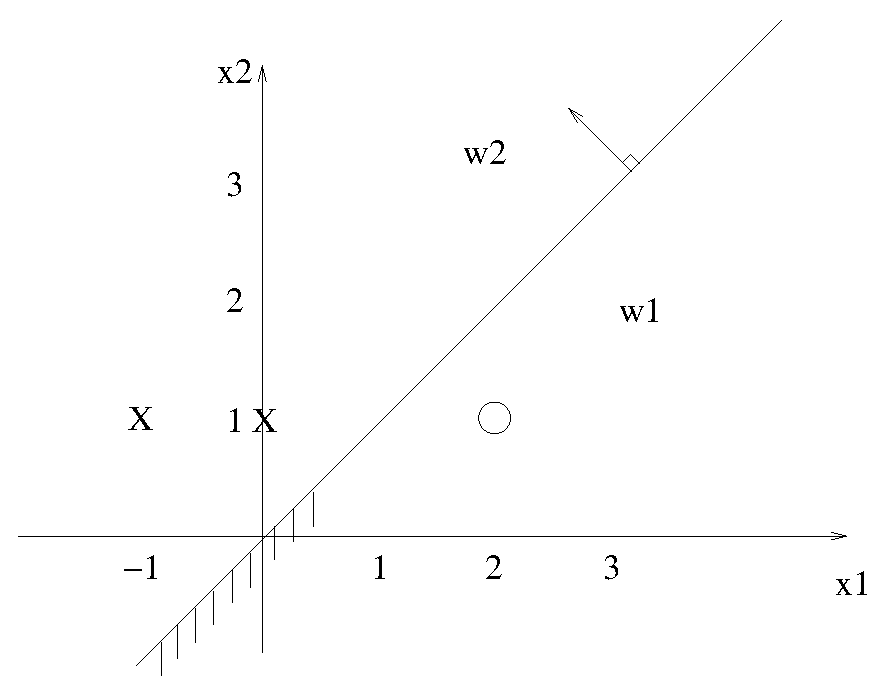
\includegraphics[scale=0.35]{e4_5.eps}
      \end{center}

      Classifications are carried out as follows:
      \begin{equation*}
        \left\{\begin{array}{l}
            \vw^T\vx<0 \Rightarrow \vx \in \omega_1\\
            \vw^T\vx\geq 0 \Rightarrow \vx \in \omega_2\\
          \end{array}\right.
      \end{equation*}

    \item

      \begin{align}
        &\omega_1:\text{\;} \{ [1,1]^T, [2,2]^T \}, \notag \\
        &\omega_2: \text{\;} \{ [1,2]^T,[2,1]^T \} \notag
      \end{align}
      \begin{center}
        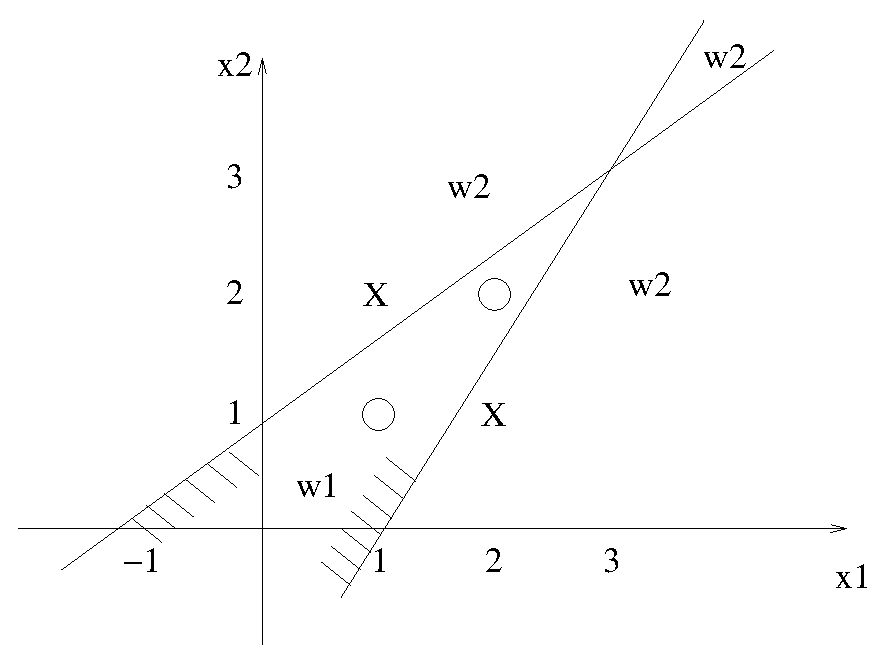
\includegraphics[scale=0.35]{e4_5b.eps}
      \end{center}

      It is not possible to separate the classes with a single
      hyperplane. At least two hyperplanes are required to separated the
      classes correctly.

    \end{enumerate}

  \end{solution}
  
\item

  a) By substituting (2.27) into (2.25) prove that
  \begin{equation*}
    J(\mathbf{w}^*) = \frac{1}{2} \mathrm{E}\{ d^2(k) \} - \frac{1}{2}
    \mathbf{p}^T \mathbf{w}^*
  \end{equation*}
  
  b) Using the equation derived in part (a), prove that (2.25) can be
  expressed as
  \begin{equation*}
    J(\mathbf{w}) = J(\mathbf{w}^*) + \frac{1}{2}( \mathbf{w} -
    \mathbf{w}^*)^T \mathbf{C}_x (\mathbf{w} - \mathbf{w}^*)
  \end{equation*}

  \begin{solution}
    
    \begin{align*}
      J(\vw)&=\frac{1}{2}E[e^2(n)]=\frac{1}{2}E[(d(n)-\mathbf{x}(n)^T\vw)^2] \\
      &=
      \frac{1}{2} E[d(n)^2] - \vw^T E[ d(n) \mathbf{x}(n)  ]  + 
      \frac{1}{2} \vw^T E[\textbf{x}(n) \textbf{x}(n)^T ] \vw \mbox{.}
    \end{align*}
    % 
    Now if we define 
    \begin{equation*}
      \textbf{C}_x = E[\textbf{x}(n) \textbf{x}(n)^T ]
    \end{equation*}
    and
    \begin{equation*}
      \textbf{p} = E[d(n) \textbf{x}(n) ] \mbox{,}
    \end{equation*}
    then
    \begin{align*}
      J(\vw) = \frac{1}{2} E[d(n)^2] - \vw^T \textbf{p}  + 
      \frac{1}{2} \vw^T \textbf{C}_x \vw \mbox{.}
    \end{align*}
    % 
    The gradient of this is
    \begin{align*}
      \nabla J =   \textbf{C}_x \vw - \textbf{p} \mbox{.}
    \end{align*}
    % 
    Now setting this to zero, we can solve for the minimizer of $J$:
    \begin{equation*}
      \textbf{w}^* = \textbf{C}_x^{-1} \textbf{p} \mbox{.}
    \end{equation*}
    Now 5(a) is solved by substituting $\textbf{w}^*$ into the expression for $J$.
    5(b) follows by a straightforward calculation or alternatively, we may observe
    that $\nabla_{\textbf{w}^*} J = 0$ and the Hessian of $J$ at $\textbf{w}^*$ is $\textbf{C}_x$.
    The higher order derivatives are zero, because $J$ is a second order polynomial with respect
    to $\textbf{w}$ and thus
    \begin{equation*}
      J(\vw) = J( \textbf{w}^* ) + \frac{1}{2} ( \vw - \textbf{w}^* ) \textbf{C}_x ( \vw - \textbf{w}^* ) \mbox{.}
    \end{equation*}

  \end{solution}
  
\end{enumerate}

\end{document}             % End of document.

%%% Local Variables: 
%%% mode: latex
%%% TeX-master: "ex02_solutions"
%%% End: 
